% ACL-format submission version of ../main.tex. Compile from this directory:
%   pdflatex main && bibtex main && pdflatex main && pdflatex main
% Numbers in Sections 5.1-5.3 and 5.5 are on the 300-question development split. The pre-registered held-out
% confirmation (protocols/main_confirmation_v1.md, scripts/23_confirm_main.py) fills Table~\ref{tab:confirm}; cells
% marked \tbd are pending that single scoring run.
\documentclass[11pt]{article}
\usepackage[review]{acl}
\usepackage{times}
\usepackage{latexsym}
\usepackage[T1]{fontenc}
\usepackage[utf8]{inputenc}
\usepackage{microtype}
\IfFileExists{inconsolata.sty}{\usepackage{inconsolata}}{}
\usepackage{graphicx}
\usepackage{amsmath,amssymb}
\usepackage{booktabs}
\usepackage{xcolor}
\graphicspath{{../figures/}}

\newcommand{\tbd}{\textcolor{red}{\textbf{tbd}}}
\newcommand{\search}{\texttt{Search}}
\newcommand{\finish}{\texttt{Finish}}

\title{Where Does an Agent Go Wrong? Step-Level Confidence\\from Internal States in Multi-Step LLM Agents}
\author{Anonymous ACL submission}

\begin{document}
\maketitle

\begin{abstract}
LLM agents fail in the middle of a trajectory, yet most uncertainty estimates are computed once, for a final answer.
We study confidence at the level of individual agent steps. ReAct agents built on Qwen2.5-7B-Instruct and
Llama-3.1-8B-Instruct answer HotpotQA questions by searching a fixed set of paragraphs, and every step receives an
automatic correctness label. We ask three questions. (1)~Which signal best detects a wrong step? A linear probe on
mid-to-late hidden states, read after the action is written, reaches AUROC 0.835 and 0.878, ahead of sampling
consistency (0.732, 0.773), a classifier on the visible action text and history (0.745, 0.746), verbalized
confidence and token log-probability; the advantage comes from search steps, and a probe read before the step is
generated still beats step position. (2)~Which errors does a probe trained on another task detect? In a
pre-registered study confirmed on 600 held-out questions per model, a probe trained to judge document choice
detects distractor retrievals better than one trained on closed-book answer correctness (+0.13 and +0.07 AUROC),
while neither is clearly better on final answers: what a transferred probe detects depends on what its source
labels measure. (3)~Are step errors coupled? A Bayesian model with a previous-error term is preferred under
PSIS-LOO, but for Qwen the coupling is largely question difficulty. Marginalising the unknown previous error repairs
the severe underconfidence of multiplied step confidences, but is not better than the last step's confidence alone.
\end{abstract}

\section{Introduction}
A multi-step agent can retrieve the wrong document, repeat a search, or commit to an answer too early, and a single
confidence score for the final answer says nothing about where things went wrong. For agents to hand control to a
person at the right moment, confidence must be estimated at each step and then aggregated over the trajectory.

Three gaps motivate this study. First, most uncertainty methods for LLMs, such as semantic entropy
\citep{kuhn2023semantic,farquhar2024detecting}, self-consistency \citep{wang2023selfconsistency} and verbalized
confidence \citep{xiong2024can}, were designed for single answers. Second, hidden-state probes predict the truth of
statements \citep{azaria2023internal,marks2023geometry}, the correctness of chain-of-thought steps
\citep{ni2026reprobe}, and the success of whole agent trajectories \citep{mammen2026agents}, but whether a probe
trained on ordinary QA transfers to agent steps is listed as an open question \citep{lin2026uqagents}, and
representation-based detectors are known to fail out of distribution \citep{dubanowska2025representation}. Third,
multiplying step-level probabilities assumes independent steps, while step errors in agents are positively coupled
\citep{lin2026uqagents}.

Our contributions are:
(i)~an offline agent benchmark with automatic step labels and four step-level signals, for two models;
(ii)~evidence that hidden-state probes detect wrong steps better than output-based signals, step position and the
visible action text, mainly on retrieval steps, and carry part of this signal before the step is written;
(iii)~a pre-registered, held-out test of \emph{what} transfers from single-step QA: the error types a transferred
probe detects follow the content of its source labels, and conclusions drawn from a single source-selected layer
do not replicate, while an average over upper layers does; and
(iv)~a Bayesian comparison of coupled and independent step-error models, showing that marginalising the coupling
avoids the underconfidence of multiplied step confidences without beating the last step's confidence.

\begin{table*}[t]
\centering\small
\caption{Step-level detection on the development test split (Qwen: 902 steps, 68.5\% correct; Llama: 1028 steps,
68.2\% correct). $\Delta$ = AUROC gap to the action-token probe with 95\% episode-bootstrap CI. Probe layers chosen
on the training split: Qwen layer 20 of 28 (mean pooling); Llama layer 23 of 32 (last token) for action tokens and
18 for the earlier points. Visible text: step index, action type, query repetition, overlap with earlier queries
and retrieved titles, argument length, answer seen in an earlier observation. Held-out confirmation:
Table~\ref{tab:confirm}.}
\label{tab:rq1}
\begin{tabular}{@{}lcccc@{}}
\toprule
& \multicolumn{2}{c}{Qwen2.5-7B} & \multicolumn{2}{c}{Llama-3.1-8B} \\
\cmidrule(lr){2-3}\cmidrule(l){4-5}
Signal & AUROC & $\Delta$ [95\% CI] & AUROC & $\Delta$ [95\% CI] \\
\midrule
Probe: action tokens & \textbf{0.835} & -- & \textbf{0.878} & -- \\
Probe: before action & 0.788 & $-0.046$ [$-0.072$, $-0.022$] & 0.791 & $-0.087$ [$-0.112$, $-0.063$] \\
Probe: before step & 0.778 & $-0.056$ [$-0.083$, $-0.031$] & 0.795 & $-0.084$ [$-0.110$, $-0.058$] \\
Sampling consistency & 0.732 & $-0.102$ [$-0.136$, $-0.067$] & 0.773 & $-0.106$ [$-0.140$, $-0.071$] \\
Verbalized confidence & 0.589 & $-0.246$ [$-0.298$, $-0.197$] & 0.701 & $-0.177$ [$-0.212$, $-0.143$] \\
Token log-prob (mean) & 0.556 & $-0.278$ [$-0.322$, $-0.237$] & 0.496 & $-0.382$ [$-0.421$, $-0.343$] \\
\midrule
Visible text + history & 0.745 & $-0.090$ [$-0.126$, $-0.056$] & 0.746 & $-0.133$ [$-0.168$, $-0.101$] \\
Step index & 0.696 & $-0.139$ [$-0.171$, $-0.107$] & 0.675 & $-0.204$ [$-0.236$, $-0.172$] \\
Step index + action type & 0.693 & $-0.142$ [$-0.178$, $-0.106$] & 0.686 & $-0.193$ [$-0.228$, $-0.160$] \\
\bottomrule
\end{tabular}
\end{table*}

\section{Related Work}
\textbf{Uncertainty for single answers.} Sampling-based methods measure agreement among generations
\citep{wang2023selfconsistency} or their semantic entropy \citep{kuhn2023semantic,farquhar2024detecting};
verbalized confidence asks the model directly \citep{xiong2024can}. All target one answer; we use their step-level
analogues as baselines.

\textbf{Probing internal states.} Linear probes on hidden states predict whether a statement is true
\citep{azaria2023internal,marks2023geometry}. ReProbe trains a small probe to judge reasoning steps
\citep{ni2026reprobe}, and \citet{mammen2026agents} predict whether a coding or database agent will eventually
succeed. We label individual tool-use steps, compare read-out points before and after the action, and control for
step position, the visible action text and question difficulty \citep{esfandyari2026disentangling}.

\textbf{Uncertainty in agents.} \citet{lin2026uqagents} survey agent uncertainty and list QA-to-agent probe
transfer and coupled step errors as open problems; representation-based detectors are known to degrade out of
distribution \citep{dubanowska2025representation}. We test transfer with a pre-registered source-swap design and
model coupling explicitly.

\section{Setup}
\textbf{Environment.} We use the distractor setting of HotpotQA \citep{yang2018hotpotqa}: each question comes with
ten paragraphs, two of which are supporting. The agent follows ReAct \citep{yao2023react} with two actions:
\search{}\texttt{[q]} returns the best-matching paragraph (exact title match, otherwise BM25), and
\finish{}\texttt{[a]} ends the episode. Episodes are capped at six steps.

\textbf{Data roles.} A development set of 900 validation questions (600 train, 300 test) was used to build and
analyse the methods. A held-out set of 600 further questions (\emph{final}) was drawn once by a fixed hash order
after excluding the development questions and any question whose normalised text is identical or near-identical
(TF-IDF cosine $\ge0.8$) to a development, TriviaQA or 2WikiMultihopQA question (Appendix~\ref{app:heldout}). It
was used only for the pre-registered tests below.

\textbf{Step labels.} A \search{} is correct if it returns a supporting paragraph not retrieved before; a
\finish{} is correct if its token F1 with the gold answer is at least 0.5; unparsable actions are incorrect.
No judge model is needed. An episode succeeds if its final answer is correct.

\textbf{Signals.} For every step we record: hidden states of eight evenly spaced layers, mean-pooled over the
action tokens and at the last action token (teacher-forced, i.e.\ once the action is written and before the tool
runs); the mean and minimum token log-probability of the action; sampling consistency, the share of five sampled
alternatives ($T=0.7$) whose action is equivalent to the greedy one (two searches are equivalent if they return the
same paragraph); and verbalized confidence, a 0--100 rating from the same model in a separate prompt.

\textbf{Models.} Qwen2.5-7B-Instruct \citep{qwen2024qwen25} and Llama-3.1-8B-Instruct \citep{grattafiori2024llama3},
both in 4-bit NF4 on a single 12\,GB GPU, with identical prompts, questions and settings. On the development
split the Qwen agent takes 3.0 steps per question, succeeds on 60.7\% of test questions and leaves 4.7\% of test
episodes unanswered; the Llama agent takes 3.4 steps, succeeds on 70.0\% and leaves 10.3\% unanswered.

\section{Methods}
\textbf{Probes.} A probe is standardisation, PCA to 64 dimensions and logistic regression. Pooling and layer are
chosen by out-of-fold AUROC on the training split, with folds grouped by question. Output-based signals are mapped
to probabilities by Platt scaling \citep{platt1999probabilistic} on the training split. Position baselines are
logistic regressions on the one-hot step index, with or without the action type; the visible-text baseline is a
logistic regression on the features listed under Table~\ref{tab:rq1}. All are fitted on the training split.

\textbf{Earlier read-out points.} Replaying each recorded trajectory, we also read the residual stream at the last
token of ``\texttt{Thought $t$:}'' (before the step) and at the last token before ``\texttt{Action $t$:}''
(after the thought, before the action).

\textbf{Transfer.} The model answers 2000 TriviaQA questions \citep{joshi2017triviaqa} closed-book; a probe trained
on the answer-span states is applied to agent steps without agent labels for its weights, and after Platt scaling
on 50 agent steps; its read-out is the agent probe's, or the best by five-fold AUROC on TriviaQA.

\textbf{Source swap.} To ask \emph{which} agent errors a transferred probe detects, we vary what the source labels
measure. S0 labels closed-book answer correctness (TriviaQA, as above). S2-QA labels document choice: given a
2WikiMultihopQA question \citep{ho2020constructing} and the titles of its ten paragraphs, the model names the
paragraph to read first (or, after one gold paragraph is shown, the next one), and the label is whether that
paragraph is supporting and new, the same rule as for agent searches. C1 asks the TriviaQA questions in the ReAct
format and isolates the prompt format. Each source is balanced to $m$ positives and $m$ negatives
($m=446$ and $693$). Target scores are \emph{same-step} AUROCs, comparing only correct and wrong steps at the same
step index, for two contrasts: \finish{} steps, and correct searches against \emph{distractor} searches that
return a new non-supporting paragraph. The pre-registered quantities are the retrieval gain
$G=A_\text{dis}(\text{S2-QA})-A_\text{dis}(\text{S0})$, the finish cost
$C=A_\text{fin}(\text{S2-QA})-A_\text{fin}(\text{S0})$ and the interaction $I=G-C$.

\textbf{Coupled step errors.} Let $s_t$ be the out-of-fold probe logit of step $t$, $k_t$ its action type, and
$e_{t-1}=1-y_{t-1}$ an error at the previous step ($e_0=0$). We compare
\begin{align*}
\text{M0: } & \operatorname{logit} P(y_t=1) = a_{k_t} + b_{k_t} s_t,\\
\text{M1: } & \operatorname{logit} P(y_t=1) = a_{k_t} + b_{k_t} s_t + g\, e_{t-1},
\end{align*}
with $\mathcal{N}(0,2^2)$ priors, fitted in PyMC \citep{abrilpla2023pymc} and compared by PSIS-LOO
\citep{vehtari2017practical} through the signal ratio $\mathrm{SR}=\Delta\mathrm{ELPD}/\mathrm{SE}$
\citep{shi2026bayesian}. At test time $y_{t-1}$ is unknown, so M1's trajectory confidence marginalises it with a
two-state forward recursion, $q_0=1$, $q_t = q_{t-1}\sigma(\eta_t) + (1-q_{t-1})\sigma(\eta_t+g)$, and $q_T$
estimates the probability that the final answer is correct. Baselines aggregate M0's step probabilities by
product, minimum, or the last step only. A hand-off policy passes an episode to a person at the first step whose
running confidence falls below $\tau$.

\textbf{Inference and pre-registration.} Gaps are full-sample point estimates with percentile intervals over 2000
resamples of whole questions, shared across the signals of one model. Both held-out analyses were written down,
with their decision rules and the mapping from outcomes to claims, before their held-out scores were computed;
inputs and code were frozen by hash, and each analysis was run once. The RQ1/RQ3 confirmation was registered after
the source-swap scoring had used the held-out step labels, but before any in-domain probe, baseline or trajectory
metric was computed on them, and it reuses the development analyses without new choices. The source-swap protocol was revised once, after the
development results and before held-out collection (Section~\ref{sec:swap}).

\begin{figure*}[t]
\centering
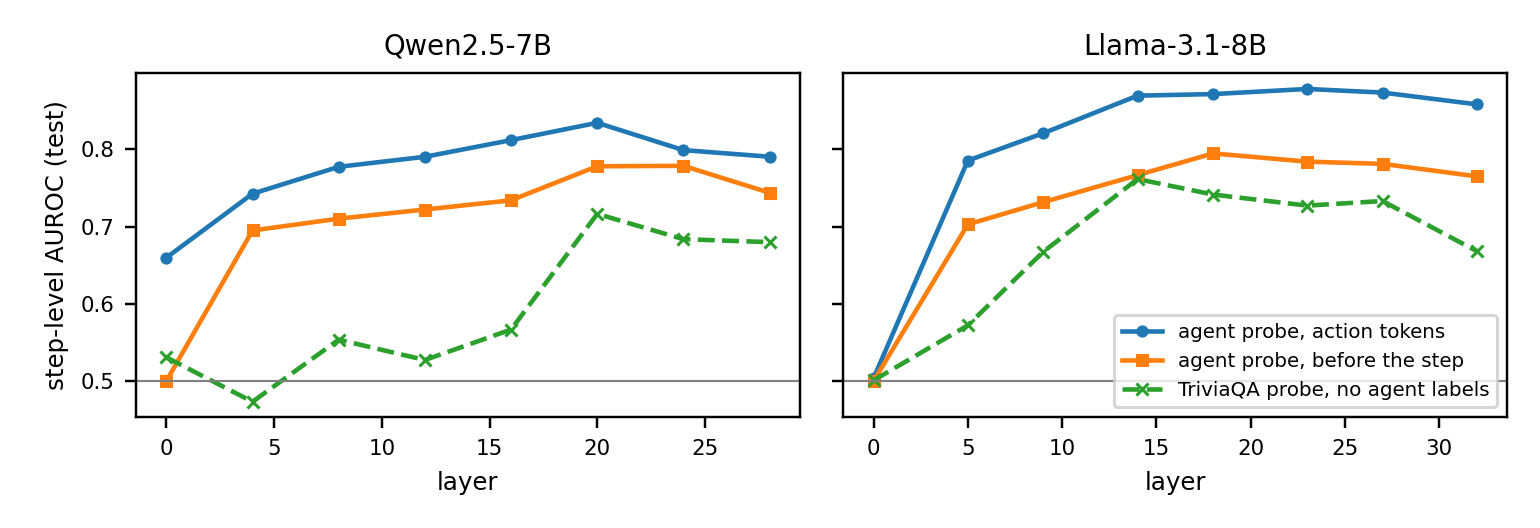
\includegraphics[width=0.68\textwidth]{layers_both.png}
\caption{Development test AUROC by layer: probes trained on agent steps (action tokens and before the step) and a
TriviaQA probe applied without agent labels. Pooling as selected for the agent probe of each model.}
\label{fig:layers}
\end{figure*}

\section{Results}
\subsection{RQ1: hidden states detect wrong steps best}
In both models the action-token probe outperforms every output-based signal by at least 0.10 AUROC
(Table~\ref{tab:rq1}), and is well calibrated (ECE 0.032 and 0.026). The advantage comes from \search{} steps
(Qwen 0.871 versus 0.751 for consistency; Llama 0.916 versus 0.803); on \finish{} steps the probe is level with
consistency (0.739 versus 0.699, gap CI [$-0.026$, 0.105]; 0.676 versus 0.692, CI [$-0.098$, 0.066]). As the probe
reads the state after the action is written, we also fit a baseline on what the agent can see. It is level with
consistency (0.745, 0.746), and the probe exceeds it by 0.090 and 0.133. On first searches, where nothing can be
repeated, the probe still reaches 0.806 and 0.845 against 0.676 and 0.753 for consistency. Verbalized confidence is
compressed: 46\% (Qwen) and 51\% (Llama) of steps are rated 80. Token log-probability is weak overall, and for
Llama's searches it ranks in the wrong direction (AUROC 0.378). Detection peaks about two-thirds of the way up the
network (Fig.~\ref{fig:layers}). Most of the signal is present before the step is generated: a probe on the state
before ``\texttt{Thought $t$:}'' reaches 0.778 and 0.795 from a single forward pass. The ranking is unchanged under
a lenient label that does not penalise repeated searches (probe versus consistency: 0.774 versus 0.692; 0.799
versus 0.732).

\subsection{Controlling for step position}
Later searches are more often repeats, so position alone predicts errors (Table~\ref{tab:rq1}). The action-token
probe beats step index and action type by 0.142 (CI [0.106, 0.178]) and 0.193 (CI [0.160, 0.228]), adding position
to the probe changes AUROC by at most 0.002, and within each step index the probe keeps AUROC 0.77--0.85 (Qwen) and
0.81--0.89 (Llama). Before the action is known, the fair baseline is step index alone; the pre-step probe adds
0.079 (CI [0.055, 0.103]) and 0.116 (CI [0.090, 0.140]) to it. Within a step index, however, the pre-step probe is
roughly level with consistency (Qwen 0.66--0.72 versus 0.68--0.74; Llama 0.71--0.81 versus 0.64--0.77), and on
late searches ($t\ge3$) it is close to chance (0.50--0.64). Part of its overall advantage over consistency is
therefore positional.

\subsection{Steps within the same question}
Pooled AUROC mostly compares steps from different questions, so it may partly reflect question difficulty
\citep{esfandyari2026disentangling}. We therefore also pool only the pairs of one correct and one wrong step from
the same trajectory (Qwen: 134 of 300 questions have both labels, 368 pairs; Llama: 137, 502 pairs). Probe AUROC
falls by 0.07 and 0.09, but stays above consistency and above step index (Table~\ref{tab:within}), and keeps
0.74--0.80 after its logit is residualised on step index and action type. Weighting questions equally gives 0.789
and 0.780 against 0.697 and 0.686 for consistency (gap CI [0.043, 0.141]; [0.046, 0.143]).

\begin{table}[t]
\centering\small
\caption{Within-question AUROC (development test): correct/wrong step pairs from one trajectory, 95\%
question-bootstrap CI. Residualised: probe logit minus a least-squares fit on step index and action type.}
\label{tab:within}
\footnotesize\setlength{\tabcolsep}{3pt}
\resizebox{\columnwidth}{!}{\begin{tabular}{@{}lcc@{}}
\toprule
Signal & Qwen2.5-7B & Llama-3.1-8B \\
\midrule
Probe: action tokens & 0.764 [0.704, 0.821] & 0.793 [0.748, 0.837] \\
\quad residualised & 0.736 [0.679, 0.793] & 0.795 [0.752, 0.838] \\
\quad \search{} only & 0.751 [0.661, 0.835] & 0.822 [0.774, 0.866] \\
Consistency & 0.700 [0.642, 0.752] & 0.655 [0.590, 0.717] \\
Step index ($-t$) & 0.698 [0.622, 0.773] & 0.602 [0.533, 0.665] \\
\bottomrule
\end{tabular}}
\end{table}

\begin{table}[t]
\centering\small
\caption{Held-out confirmation of RQ1 and RQ3 (600 final questions per model; probes and baselines fitted on the
development training split). P1--P3: 98.3\% CIs (Bonferroni over three claims); others 95\%.}
\label{tab:confirm}
\footnotesize\setlength{\tabcolsep}{3pt}
\resizebox{\columnwidth}{!}{\begin{tabular}{@{}lcc@{}}
\toprule
Pre-registered gap & Qwen2.5-7B & Llama-3.1-8B \\
\midrule
P1 probe $-$ consistency & \tbd & \tbd \\
P2 probe $-$ visible text & \tbd & \tbd \\
P3 pre-step probe $-$ step index & \tbd & \tbd \\
S1 \search{}: probe $-$ consistency & \tbd & \tbd \\
S2 within question & \tbd & \tbd \\
S4 ECE product $-$ forward & \tbd & \tbd \\
S5 $g$ (90\% interval) & \tbd & \tbd \\
\bottomrule
\end{tabular}}
\end{table}

\subsection{RQ2: what a transferred probe detects}
\label{sec:swap}
\textbf{Transfer happens only from middle layers up.} A probe trained on closed-book TriviaQA answers (52\% and
65\% correct) transfers to agent steps only above a model-specific depth (Fig.~\ref{fig:layers}). For Qwen it is
near chance up to layer 16 (AUROC 0.47--0.57) and reaches 0.717 at layer 20; for Llama it stays at 0.73--0.76 from
layer 14 to 27. These read-outs were chosen on agent training labels; choosing them on TriviaQA alone gives 0.623
and 0.762. Raw probabilities are badly calibrated (ECE 0.471 and 0.248); Platt scaling on 50 agent steps reduces
this (mean ECE 0.093 and 0.122) without changing the ranking. For Qwen this matches an in-domain probe trained on
the same 50 steps (AUROC 0.731); for Llama the small in-domain probe is better (0.779).

\textbf{Which errors transfer.} On the development split the TriviaQA probe detected wrong answers about as well as
an in-domain probe but lagged it on distractor searches, suggesting that a source covers the errors its labels
measure. The source-swap study tests this. Its first pre-registered version chose one read-out per source on
source validation data; on the development split this gave $I=+0.351$ [0.224, 0.480] for Qwen but $+0.080$
[$-0.044$, 0.208] for Llama, so the interaction was not established. The layer curves showed the Llama result
hinged on all three sources selecting the same layer, where S0 happened to peak. Having seen this, we revised the
read-out rule before collecting held-out data: each source's score is the average AUROC over the eight upper-half
read-outs (four layers $\times$ two poolings), with no selection. Because the rule was chosen after seeing
development data, only the held-out test counts as evidence.

\begin{table*}[t]
\centering\small
\caption{Source swap on the 600 held-out questions per model: same-step AUROC averaged over eight upper-layer
read-outs, and the pre-registered gaps with 95\% question-bootstrap CIs. \finish: 570 / 536 steps (195 / 134
wrong); distractor: 1058 / 1235 steps (209 / 268 wrong). Last column: point estimates of $I$ / $G$ / $C$ under the
first protocol's single source-selected read-out, scored on the same data.}
\label{tab:swap}
\setlength{\tabcolsep}{4pt}
\resizebox{\textwidth}{!}{\begin{tabular}{@{}lcccccccccc@{}}
\toprule
& \multicolumn{3}{c}{$A_\text{fin}$} & \multicolumn{3}{c}{$A_\text{dis}$} & & & & Single read-out \\
\cmidrule(lr){2-4}\cmidrule(lr){5-7}
Model & S0 & C1 & S2-QA & S0 & C1 & S2-QA & $I$ (interaction) & $G$ (retrieval gain) & $C$ (finish cost) & $I$ / $G$ / $C$ \\
\midrule
Qwen & .633 & .641 & .615 & .554 & .606 & \textbf{.681} & $+$.145 [.101, .192] & $+$.127 [.094, .158] & $-$.018 [$-$.055, .018] & .190 / .065 / $-$.126 \\
Llama & .687 & .681 & .636 & .663 & .645 & \textbf{.728} & $+$.117 [.070, .162] & $+$.066 [.038, .094] & $-$.051 [$-$.086, $-$.017] & $-$.023 / $-$.033 / $-$.010 \\
\bottomrule
\end{tabular}}
\end{table*}

On the held-out questions (Table~\ref{tab:swap}) the interaction and the retrieval gain hold in both models: a
probe trained to choose documents detects distractor retrievals 0.13 and 0.07 AUROC better than one trained on
answer correctness. The finish cost is inconclusive for Qwen and a small loss for Llama ($-0.051$), so under the
pre-registered mapping we claim the retrieval gain only, not that the swap is free on final answers. Changing only
the format (C1 $-$ S0) moves finish AUROC by less than 0.01 in both models. The single-read-out rule, scored on the
same held-out data, again disagrees across models (Table~\ref{tab:swap}, last column): conclusions about transfer from
one selected layer are fragile, and averaging over the layers where transfer occurs makes them stable. A 2WikiMultihopQA
ReAct source was also planned, but the model almost never chose a wrong document in that format (2\% of
searches), too few negatives to train on (Appendix~\ref{app:swap}).

\begin{table}[t]
\centering\small
\caption{Trajectory confidence on finished development test episodes (Qwen: 286, 63.6\% correct; Llama: 269, 78.1\%
correct). ECE: ten equal-width bins.}
\label{tab:rq3}
\footnotesize\setlength{\tabcolsep}{2.6pt}
\resizebox{\columnwidth}{!}{\begin{tabular}{@{}lcccccc@{}}
\toprule
& \multicolumn{3}{c}{Qwen2.5-7B} & \multicolumn{3}{c}{Llama-3.1-8B} \\
\cmidrule(lr){2-4}\cmidrule(l){5-7}
Aggregation & AUROC & ECE & Brier & AUROC & ECE & Brier \\
\midrule
M1 forward & 0.735 & \textbf{0.027} & 0.193 & 0.682 & 0.104 & \textbf{0.170} \\
M0 last step & 0.739 & 0.057 & \textbf{0.192} & 0.676 & \textbf{0.096} & \textbf{0.170} \\
M0 minimum & 0.702 & 0.082 & 0.212 & 0.659 & 0.206 & 0.230 \\
M0 product & 0.664 & 0.200 & 0.260 & 0.642 & 0.326 & 0.299 \\
\bottomrule
\end{tabular}}
\end{table}

\subsection{RQ3: coupling is partly question difficulty}
M1 is preferred to M0 in both models (Qwen: $\Delta$ELPD $=5.58$, SE $=3.75$, SR $=1.49$, all Pareto $k<0.16$;
Llama: $\Delta$ELPD $=7.22$, SE $=4.17$, SR $=1.73$, maximum Pareto $k=0.76$, so the Llama comparison needs
caution). The coupling coefficients agree closely: $g=-0.58$ $[-0.84,-0.33]$ and $g=-0.62$ $[-0.87,-0.37]$ (90\%
intervals): after an error, the odds that the next step is correct fall to about 0.55 of their value, even given
the probe signal. This is a conditional association, not propagation. Hard questions could also cause runs of
errors. With a question random intercept, $g$ is $-0.44$ $[-0.76,-0.10]$ for Qwen and $-0.59$ $[-0.85,-0.33]$ for
Llama, but PSIS-LOO then prefers M1 only for Llama (SR $-0.87$ and 1.32). Multiplying step confidences badly
underestimates success (mean confidence 0.44 and 0.45 versus 63.6\% and 78.1\% observed), because a wasted search
is often recovered. The forward recursion removes most of this error (ECE 0.027 versus 0.200, gap CI [0.082,
0.186]; 0.104 versus 0.326, CI [0.189, 0.244]; Table~\ref{tab:rq3}). Its calibration, however, does not differ
significantly from the last step alone (ECE gap last $-$ forward 0.030, CI [$-0.030$, 0.055]; $-0.008$, CI
[$-0.024$, 0.033]), and it does not rank episodes better (AUROC gap $-0.004$, CI [$-0.017$, 0.009]; $+0.006$, CI
[$-0.015$, 0.028]). The hand-off curve of M1 lies at or above that of M0's running product
(Fig.~\ref{fig:handoff}), but the difference in area under the risk--coverage curve is not significant (0.019, CI
[$-0.003$, 0.041]; 0.005, CI [$-0.010$, 0.020]), and the same first-drop rule on M0's current-step probability
matches M1, so the gap comes from the aggregation rule, not the history term.

\begin{figure}[t]
\centering
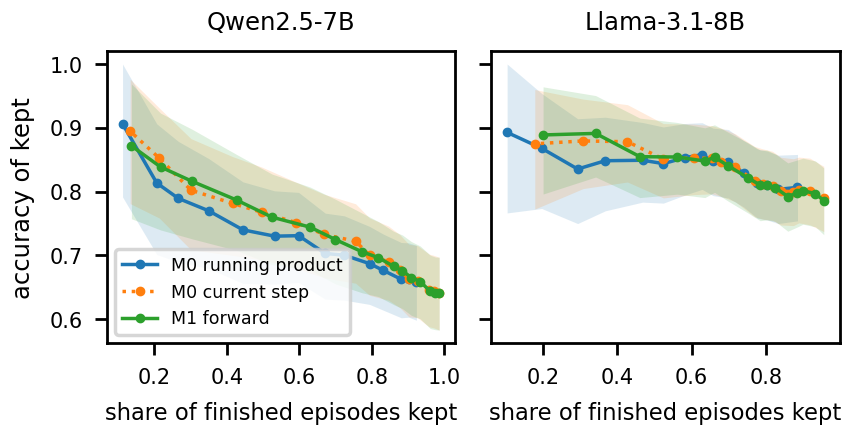
\includegraphics[width=\columnwidth]{handoff_both.png}
\caption{Hand-off on finished development test episodes at the first step whose running quantity falls below
$\tau$. Bands: 95\% episode bootstrap; points keeping under 10\% are omitted.}
\label{fig:handoff}
\end{figure}

\section{Discussion}
Internal states carry information about step correctness that output-based signals, step position and the visible
action text miss, concentrated on retrieval steps; judging a final answer remains as hard for the probe as for
sampling. The source-swap results sharpen the transfer picture: a probe trained elsewhere is not a generic
``something is wrong'' detector, and which agent errors it covers follows what its source labels measure. Two
methodological lessons generalise. First, transfer conclusions drawn from a single read-out selected on source data
can reverse between models and splits; averaging over the layers where transfer occurs is more stable. Second,
multiplying step confidences is a poor trajectory estimate in agents that recover from wasted steps, but modelling
the coupling explicitly does not beat simply trusting the last step.

\section*{Limitations}
The study uses one environment (HotpotQA with a fixed paragraph set), one seed and two 7--8B models in 4-bit
precision; longer-horizon or interactive environments and larger models may behave differently. Step labels are
automatic and conservative: a repeated search counts as wrong and a final answer is judged by token F1, and we have
not yet completed a manual audit of the labels. RQ1 and RQ3 figures in the main text come from a 300-question
development split that was analysed repeatedly; their held-out confirmation is Table~\ref{tab:confirm}. The
source-swap read-out rule was fixed after seeing development data, which is why only the held-out test is counted
as evidence; its conclusions are limited to HotpotQA, and we do not claim that the finish cost is negligible.
Trajectory-level results on the development split use finished episodes only; the excluded unfinished episodes
(4.7\% and 10.3\%) are all failures, so kept accuracy in the hand-off curves is optimistic. Hand-offs are simulated
on recorded trajectories; we have not intervened online, and the effect of replanning or human takeover cannot be
inferred from these logs.

\section*{Ethics Statement}
We use public research datasets (HotpotQA, TriviaQA, 2WikiMultihopQA) and openly released models under their
licences; no human subjects or personal data are involved. Step-level confidence is meant to support handing
control to a person; a miscalibrated estimate could instead hide errors, so deployed thresholds should be validated
on the target task.

\bibliography{../refs}

\appendix

\section{Held-out question selection}
\label{app:heldout}
The pool is the HotpotQA distractor validation set at a pinned revision (7,405 questions). We excluded the 900
development questions, duplicates within the pool, and any question whose normalised text matched, or had TF-IDF
cosine $\ge0.8$ (word 1--2 grams) with, a development question, any of the 9,960 TriviaQA validation questions or
any of the 12,576 2WikiMultihopQA development questions. No question was excluded as a near-duplicate; the largest
remaining cosine is 0.48. Questions were ordered by $\mathrm{sha256}(\texttt{"heldout-v1:"}+\mathrm{id})$; the
first 200 form a calibration split not used here and the next 600 the final split. Selection reads only question
IDs and text, and a verification script re-derives the manifest from the raw files.

\section{Source-swap details}
\label{app:swap}
\textbf{Labels.} S2-QA asks ``which document should be read first?'' and parses one title; it is correct if the
title is a supporting paragraph not yet shown. Half of the items are second-hop decisions whose history shows one
gold paragraph. Title matching ignores diacritics, because 8.7\% of 2WikiMultihopQA supporting titles contain
non-ASCII characters that the models often drop. A ReAct-format variant (S2) was dropped after a 50-question pilot:
only 2 of 96 searches were wrong.

\textbf{Balancing and fitting.} Each source is ordered by a salted hash; the first $m$ positives and $m$ negatives
form the training sample, where $m$ is the smallest class count across the three sources. Probes use the same
architecture as the agent probe and are fitted on all $2m$ items; no agent label is used.

\textbf{Exploratory.} On the held-out split, the distractor gain S2-QA $-$ S0 is positive in 15 of the 16
individual upper-layer read-outs across the two models (Qwen 0.13--0.17 except mean-pooled layer 28 at $-0.004$;
Llama 0.005--0.13).

\end{document}
